\newcommand{\TaylorApproximationVisual}{%
\begin{center}
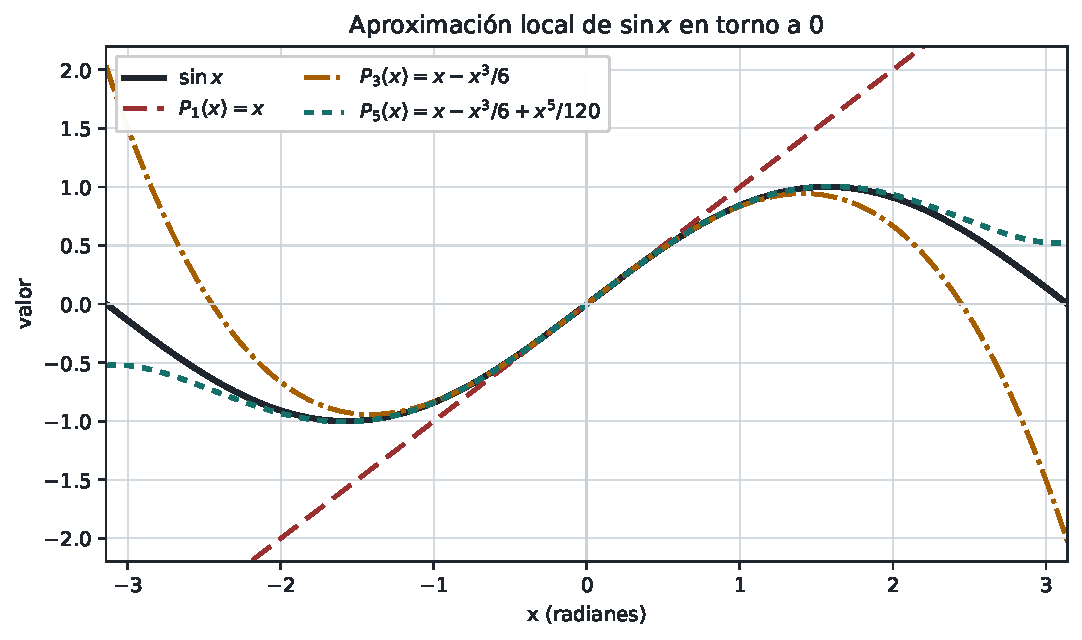
\includegraphics[width=0.94\linewidth]{src/theory/assets/plots/taylor_approximation.pdf}

\small\itshape Lectura del gráfico: cerca de cero, los polinomios de mayor
grado siguen al seno durante un intervalo más amplio. La comparación sigue
siendo local; no afirma una igualdad global.
\end{center}%
}

\newcommand{\TaylorErrorVisual}{%
\begin{center}
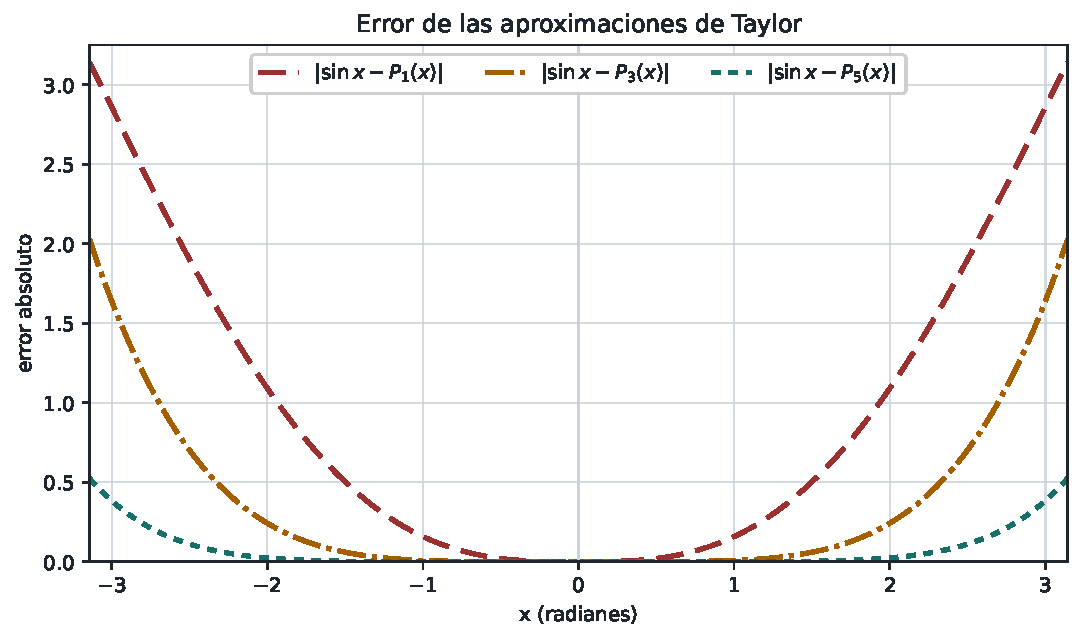
\includegraphics[width=0.94\linewidth]{src/theory/assets/plots/taylor_error.pdf}

\small\itshape Lectura del gráfico: el error se anula en el centro y crece al
alejarse. Comparar grados requiere fijar el mismo punto o intervalo; la forma
de las curvas hace visible esa condición.
\end{center}%
}
